\chapter{Searching Algorithms}

This chapter explains fundamental searching algorithms with step-by-step examples, complete C++ implementations using the \texttt{listings} package, and diagrams illustrating the search process.

\section{Linear Search}
Linear Search scans each element of the array sequentially until the target value is found or the end of the array is reached.

\subsection{Explanation}
Given an array \( arr \) of size \( n \) and a target value, the algorithm starts at the first element and compares each element with the target. If a match is found, the index is returned; otherwise, it continues until all elements are checked.

\subsection{C++ Code Example}
\begin{lstlisting}[language=C++, caption={Linear Search Implementation}]
#include <bits/stdc++.h>
using namespace std;

int linearSearch(const vector<int>& arr, int target) {
    for (int i = 0; i < arr.size(); i++) {
        if (arr[i] == target)
            return i; // Target found at index i
    }
    return -1; // Target not found
}
int main() {
    vector<int> arr = {3, 8, 2, 5, 9, 1};
    int target = 5;
    int index = linearSearch(arr, target);
    if (index != -1)
        cout << "Target " << target << " at index " << index << "\n";
    else
        cout << "Target " << target << " not found." << "\n";
        
    return 0;
}
\end{lstlisting}

\subsection{Diagram: Linear Search Process}
The following diagram shows how Linear Search traverses the array sequentially.

\begin{figure}[H]
\centering
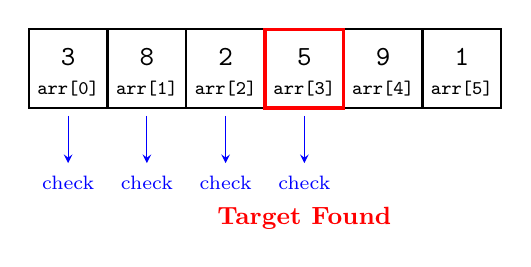
\begin{tikzpicture}[>=stealth, node distance=1.2cm]
  % Draw array boxes with values
  \foreach \i/\val in {0/3, 1/8, 2/2, 3/5, 4/9, 5/1} {
    \draw[thick] (\i,0) rectangle (\i+1,1);
    \node at (\i+0.5,0.65) {\texttt{\val}};
    \node at (\i+0.5,0.25) {\scriptsize\texttt{arr[\i]}};
  }

  % Highlight target element (assume target is at index 3)
  \draw[very thick, red] (3,0) rectangle (4,1);

  % Draw arrows and labels below each element checked
  \foreach \i in {0,...,3} {
    \draw[->, blue] (\i+0.5, -0.1) -- (\i+0.5, -0.7);
    \node[blue] at (\i+0.5, -0.95) {\scriptsize check};
  }

  % Target found text
  \node[red, font=\small\bfseries] at (3.5, -1.4) {Target Found};
\end{tikzpicture}
\caption{Linear Search: Sequentially checking each element}
\end{figure}


\section{Binary Search}
Binary Search is a highly efficient algorithm for searching in a sorted array. It repeatedly divides the search interval in half.

\subsection{Explanation}
Given a sorted array \( arr \) of size \( n \) and a target value, Binary Search works as follows:
\begin{enumerate}
  \item Set two pointers, \( \text{low} = 0 \) and \( \text{high} = n-1 \).
  \item Find the middle index: \( \text{mid} = \lfloor (\text{low} + \text{high})/2 \rfloor \).
  \item If \( arr[\text{mid}] \) equals the target, return \( \text{mid} \).
  \item If the target is less than \( arr[\text{mid}] \), repeat the search in the left subarray.
  \item Otherwise, repeat the search in the right subarray.
\end{enumerate}

\subsection{C++ Code Example}
\begin{lstlisting}[language=C++, caption={Binary Search Implementation}]
#include <bits/stdc++.h>
using namespace std;

int binarySearch(const vector<int>& arr, int target) {
    int low = 0, high = arr.size() - 1;
    while (low <= high) {
        int mid = low + (high - low) / 2;
        if (arr[mid] == target)
            return mid; // Target found
        else if (arr[mid] < target)
            low = mid + 1;
        else
            high = mid - 1;
    }
    return -1; // Target not found
}
int main() {
    vector<int> arr = {1, 3, 5, 7, 9, 11};
    int target = 7;
    int index = binarySearch(arr, target);
    if (index != -1)
        cout << "Target " << target << " at index " << index << "\n";
    else
        cout << "Target " << target << " not found." << "\n";
    return 0;
}
\end{lstlisting}

\subsection{Diagram: Binary Search Process}
The following diagram illustrates how Binary Search halves the search interval at each step.

\begin{figure}[H]
\centering
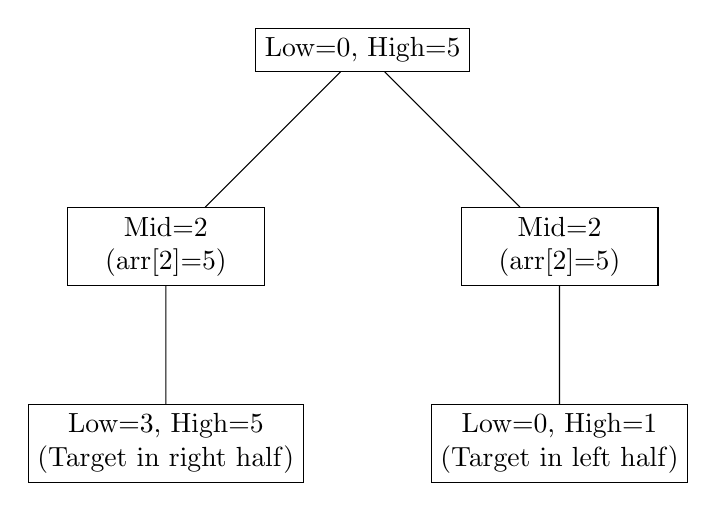
\begin{tikzpicture}[grow=down, level distance=2.5cm, sibling distance=5cm,
  every node/.style={draw, rectangle, align=center, minimum width=2.5cm}]
  \node {Low=0, High=5}
    child { node {Mid=2\\(arr[2]=5)} 
      child { node {Low=3, High=5\\(Target in right half)} } }
    child { node {Mid=2\\(arr[2]=5)} 
      child { node {Low=0, High=1\\(Target in left half)} } };
\end{tikzpicture}
\caption{Binary Search: Halving the search interval}
\end{figure}

\subsection{Step-by-Step Example of Binary Search}
Consider a sorted array: \([1, 3, 5, 7, 9, 11]\) and a target value of 7.
\begin{enumerate}
  \item Initialize: \(\text{low} = 0\), \(\text{high} = 5\). Compute \(\text{mid} = 2\). \(arr[2] = 5\). Since \(5 < 7\), move to the right half.
  \item Update: \(\text{low} = 3\), \(\text{high} = 5\). Compute \(\text{mid} = 4\). \(arr[4] = 9\). Since \(9 > 7\), move to the left half.
  \item Update: \(\text{low} = 3\), \(\text{high} = 3\). Compute \(\text{mid} = 3\). \(arr[3] = 7\). Target found at index 3.
\end{enumerate}

\section{Exponential Search}
Exponential Search is useful for unbounded or large sorted arrays. It first finds a range where the target may reside by repeatedly doubling the index, then performs a Binary Search in that range.

\subsection{Explanation}
Given a sorted array \( arr \) of size \( n \) and a target value:
\begin{enumerate}
  \item If \( arr[0] \) is the target, return index 0.
  \item Otherwise, initialize index \( i = 1 \) and double \( i \) until \( arr[i] > \) target or \( i \geq n \).
  \item Perform Binary Search on the subarray from \( i/2 \) to \( \min(i, n-1) \).
\end{enumerate}

\subsection{C++ Code Example}
\begin{lstlisting}[language=C++, caption={Exponential Search Implementation}]
#include <bits/stdc++.h>
using namespace std;

int binarySearch(const vector<int>& arr, int low, int high, int target) {
    while (low <= high) {
        int mid = low + (high - low) / 2;
        if (arr[mid] == target)
            return mid;
        else if (arr[mid] < target)
            low = mid + 1;
        else
            high = mid - 1;
    }
    return -1;
}

int exponentialSearch(const vector<int>& arr, int target) {
    int n = arr.size();
    if (n == 0) return -1;
    if (arr[0] == target) return 0;
    int i = 1;
    while (i < n && arr[i] <= target)
        i *= 2;
    return binarySearch(arr, i / 2, min(i, n - 1), target);
}
int main() {
    vector<int> arr = {1, 3, 5, 7, 9, 11, 13, 15, 17, 19};
    int target = 15;
    int index = exponentialSearch(arr, target);
    if (index != -1)
        cout << "Target " << target << " at index " << index << "\n";
    else
        cout << "Target " << target << " not found." << "\n"; 
    return 0;
}
\end{lstlisting}

\subsection{Diagram: Exponential Search Process}
The diagram below shows how the algorithm doubles the index until the range is found, then performs Binary Search.

\begin{figure}[H]
\centering
\begin{tikzpicture}[node distance=1.2cm]
    \node[draw, rectangle] (i0) {Index 0};
    \node[draw, rectangle, right=of i0] (i1) {Index 1};
    \node[draw, rectangle, right=of i1] (i2) {Index 2};
    \node[draw, rectangle, right=of i2] (i4) {Index 4};
    \node[draw, rectangle, right=of i4] (i8) {Index 8};
    \node[right=of i8] (dots) {...};
    \draw[->] (i0) -- (i1);
    \draw[->] (i1) -- (i2);
    \draw[->] (i2) -- (i4);
    \draw[->] (i4) -- (i8);
    \draw[->] (i8) -- (dots);
\end{tikzpicture}
\caption{Exponential Search: Doubling indices to find the search range}
\end{figure}

\section{Interpolation Search}
Interpolation Search improves upon Binary Search for uniformly distributed arrays by estimating the position of the target using the values at the endpoints.

\subsection{Explanation}
For a sorted array \( arr \) of size \( n \) and target value:
\[
\text{pos} = \text{low} + \frac{(target - arr[low]) \times (high - low)}{arr[high] - arr[low]}
\]
This position is used to probe the array. If the target is found at \(\text{pos}\), the index is returned; otherwise, the search continues in the appropriate subarray.

\subsection{C++ Code Example}
\begin{lstlisting}[language=C++, caption={Interpolation Search Implementation}]
#include <bits/stdc++.h>
using namespace std;

int interpolationSearch(const vector<int>& arr, int target) {
    int low = 0, high = arr.size() - 1;
    while (low <= high && target >= arr[low] && target <= arr[high]) {
        if (low == high) {
            if (arr[low] == target) return low;
            return -1;
        }
        int pos = low + ((double)(high - low) / (arr[high] - arr[low])) * (target - arr[low]);
        
        if (arr[pos] == target)
            return pos;
        if (arr[pos] < target)
            low = pos + 1;
        else
            high = pos - 1;
    }
    return -1;
}

int main() {
    vector<int> arr = {10, 20, 30, 40, 50, 60, 70, 80, 90};
    int target = 70;
    int index = interpolationSearch(arr, target);
    
    if (index != -1)
        cout << "Target " << target << " at index " << index << "\n";
    else
        cout << "Target " << target << " not found." << "\n";
        
    return 0;
}
\end{lstlisting}

\paragraph{Time Complexity Analysis:}
\begin{itemize}
  \item \textbf{Average Case:} \(O(\log \log n)\) for uniformly distributed data.
  \item \textbf{Worst Case:} \(O(n)\) when the data is not uniformly distributed.
\end{itemize}

\section{Conclusion}
In this chapter, we explored several searching algorithms:
\begin{itemize}
  \item \textbf{Linear Search}: Simple and works on unsorted data (\(O(n)\)).
  \item \textbf{Binary Search}: Efficient on sorted arrays (\(O(\log n)\)).
  \item \textbf{Exponential Search}: Finds the range for Binary Search in unbounded arrays (\(O(\log n)\)).
  \item \textbf{Interpolation Search}: Optimized for uniformly distributed data (\(O(\log \log n)\) on average).
\end{itemize}

Each algorithm has its strengths and is applicable to different scenarios. Understanding these algorithms and their performance characteristics is crucial for selecting the most appropriate method for your needs.
